\documentclass[xetex,mathserif,serif]{beamer}

\usepackage{xunicode}
\usepackage{xltxtra}
\usepackage{color}
\usepackage{url}
\usepackage{listings}
\usepackage{fontspec}
\usepackage{geometry}
\usepackage{lastpage}
\usepackage{fancyhdr}
\usepackage{amsmath}
\usepackage{amsthm}
\usepackage{amssymb}
\usepackage{blkarray}
\usepackage{multicol}
\usepackage{relsize}

\definecolor{solarized@base03}{HTML}{002B36}
\definecolor{solarized@base02}{HTML}{073642}
\definecolor{solarized@base01}{HTML}{586e75}
\definecolor{solarized@base00}{HTML}{657b83}
\definecolor{solarized@base0}{HTML}{839496}
\definecolor{solarized@base1}{HTML}{93a1a1}
\definecolor{solarized@base2}{HTML}{EEE8D5}
\definecolor{solarized@base3}{HTML}{FDF6E3}
\definecolor{solarized@yellow}{HTML}{B58900}
\definecolor{solarized@orange}{HTML}{CB4B16}
\definecolor{solarized@red}{HTML}{DC322F}
\definecolor{solarized@magenta}{HTML}{D33682}
\definecolor{solarized@violet}{HTML}{6C71C4}
\definecolor{solarized@blue}{HTML}{268BD2}
\definecolor{solarized@cyan}{HTML}{2AA198}
\definecolor{solarized@green}{HTML}{859900}
\definecolor{yaleblue}{HTML}{0E4C92}

\setbeamertemplate{navigation symbols}{}
% \setbeamerfont{title}{family=\old}
% \setbeamerfont{author}{family=\tfont}%
% \setbeamerfont{frametitle}{family=\oldA}
% \setbeamerfont{date}{family=\dfont}

\setbeamertemplate{itemize items}{--}
\setbeamercolor*{item}{fg=black}

\defaultfontfeatures{Mapping=tex-text}
\hypersetup{pdfstartview={FitH}}

\newcommand{\old}[1]{\fontspec[Alternate=1,Ligatures={Common}]{Hoefler Text}\fontsize{18pt}{30pt}\selectfont #1}%
\newcommand{\oldA}[1]{\fontspec[Alternate=1,Ligatures={Common, Rare}]{Hoefler Text}\fontsize{12pt}{15pt}\selectfont #1}%
\newcommand{\oldB}[1]{\fontspec[Ligatures={Common}]{Didot}\fontsize{12pt}{15pt}\color{solarized@base02}\selectfont #1}%
\newcommand{\tfont}[1]{\fontspec[Alternate=1,Ligatures={Common}]{Hoefler Text}\fontsize{12pt}{20pt}\selectfont #1}%
\newcommand{\dfont}[1]{\fontspec[Ligatures={Common}]{Didot}\fontsize{12pt}{12pt}\selectfont #1}%

\newcommand{\minimize}{\mathop{\mathrm{minimize}}}
\newcommand{\argmin}{\mathop{\mathrm{arg\,min}}}
\newcommand{\argmax}{\mathop{\mathrm{arg\,max}}}
\newcommand{\st}{\mathop{\mathrm{subject\,\,to}}}

\newcommand\independent{\protect\mathpalette{\protect\independenT}{\perp}}
\def\independenT#1#2{\mathrel{\rlap{$#1#2$}\mkern2mu{#1#2}}}

\setlength{\parindent}{0pt}
\setlength{\parskip}{12pt}

\setromanfont [Ligatures={Common}, Numbers={OldStyle}, Variant=01,
 BoldFont={LinLibertine_RB.otf},
 ItalicFont={LinLibertine_RI.otf},
 BoldItalicFont={LinLibertine_RBI.otf}
 ]{LinLibertine_R.otf}



\begin{document}

%%%%%%%%%%%%%%%%%%%%%%%%%%%%%%%%%%%%%%%%%%%%%%%%%%%
\begin{frame}[fragile] \frametitle{}

\vfill

{\fontsize{0.7cm}{0cm}\selectfont Lecture 14 \\\vspace{0.2cm}
Singular Value Decomposition}\\\vspace{0.5cm}
02 November 2015

\vspace{2cm}

\begin{minipage}{0.6\textwidth}
Taylor B. Arnold \\
Yale Statistics \\
STAT 312/612
\end{minipage}
\hfill
\begin{minipage}{0.3\textwidth}\raggedleft

\includegraphics[scale=0.3]{../yale-logo.png}
\end{minipage}%

\end{frame}

%%%%%%%%%%%%%%%%%%%%%%%%%%%%%%%%%%%%%%%%%%%%%%%%%%%
\begin{frame}[fragile] \frametitle{}

{\color{yaleblue}\fontsize{16pt}{20pt}\selectfont Goals for today}

\begin{itemize}
\item overview of shrinkage estimators
\item eigenvalue decomposition
\item singular value decomposition
\end{itemize}

\end{frame}

%%%%%%%%%%%%%%%%%%%%%%%%%%%%%%%%%%%%%%%%%%%%%%%%%%%
\begin{frame}[fragile] \frametitle{}

\begin{flushright}
{\color{yaleblue}\sc\fontsize{1cm}{0cm}\selectfont A bit of STAT 610}
\end{flushright}

\end{frame}


%%%%%%%%%%%%%%%%%%%%%%%%%%%%%%%%%%%%%%%%%%%%%%%%%%%
\begin{frame}[fragile] \frametitle{}

{\bf Loss}

A \textit{loss function} describes how bad an estimator $\widehat{\theta}$
is for a particular unknown parameter $\theta$. The most commonly used loss
function in statistics is the squared error loss:
\begin{align*}
\mathcal{L} (\theta, \widehat{\theta}) &= || \theta - \widehat{\theta}||_2^2
\end{align*}

\end{frame}

%%%%%%%%%%%%%%%%%%%%%%%%%%%%%%%%%%%%%%%%%%%%%%%%%%%
\begin{frame}[fragile] \frametitle{}

{\bf Risk}

A \textit{risk} of a statistical estimator is expected loss of the
estimator:
\begin{align*}
\mathcal{R} (\widehat{\theta}, \theta) &= \mathbb{E} \mathcal{L} (\theta, \widehat{\theta})
\end{align*}
\pause Notice that in general the risk is a function of the true value of
$\theta$!

\end{frame}

%%%%%%%%%%%%%%%%%%%%%%%%%%%%%%%%%%%%%%%%%%%%%%%%%%%
\begin{frame}[fragile] \frametitle{}

{\bf Admissible}

An estimator is \textit{admissible} if there is no other estimator that has
a better risk  for all values of $\theta$.

\end{frame}

%%%%%%%%%%%%%%%%%%%%%%%%%%%%%%%%%%%%%%%%%%%%%%%%%%%
\begin{frame}[fragile] \frametitle{}

Take an estimator $\widehat{p}$ for estimating the probability of observing
a $1$ in a single Bernoilli trial. \pause The estimator can be described by
exactly two numbers:
\begin{align*}
\widehat{p}(0) &= a \\
\widehat{p}(1) &= b
\end{align*}
In other words, what do you guess the probability is when you observe a $0$
and what do you guess the probability is when you observe a $1$.

\end{frame}

%%%%%%%%%%%%%%%%%%%%%%%%%%%%%%%%%%%%%%%%%%%%%%%%%%%
\begin{frame}[fragile] \frametitle{}

Is the estimator $a$ = $b$ = $0.5$ admissible?

\pause Its risk is:
\begin{align*}
\mathbb{E} \mathcal{L} (\theta, \widehat{\theta})
&= \mathbb{P}(X = 0) \cdot (p - a)^2 + \mathbb{P}(X = 1) \cdot (p - b)^2 \\
&= (1-p) \cdot (p - 0.5)^2 + p \cdot (p - 0.5)^2 \\
&= (p - 0.5)^2
\end{align*}

\end{frame}

%%%%%%%%%%%%%%%%%%%%%%%%%%%%%%%%%%%%%%%%%%%%%%%%%%%
\begin{frame}[fragile] \frametitle{}

\begin{center}
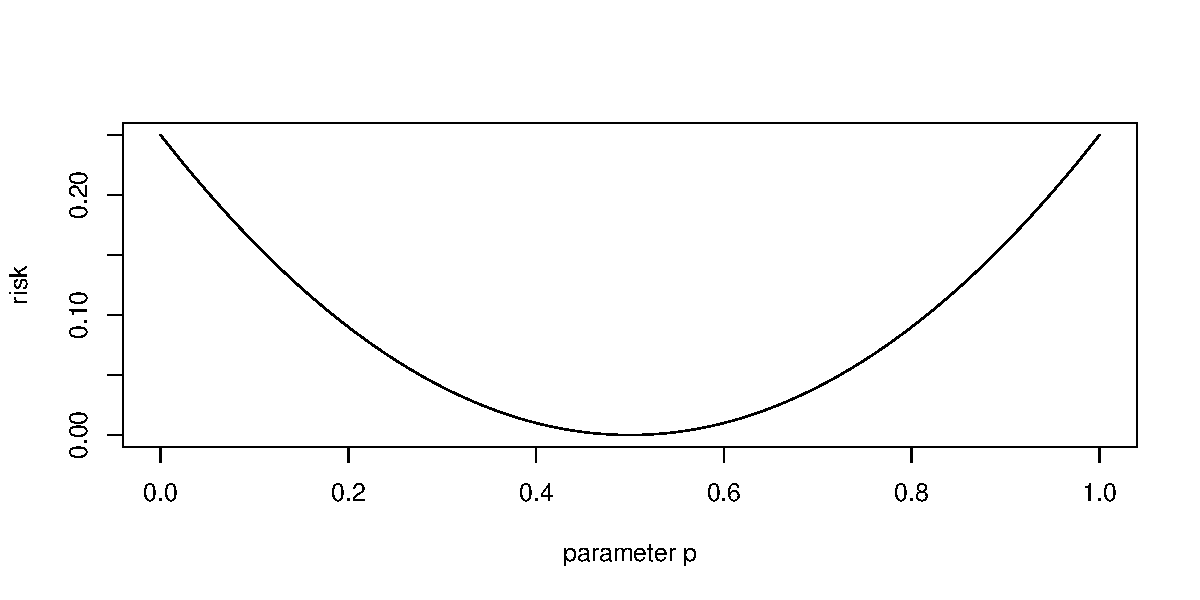
\includegraphics[width=\textwidth]{img/fig01.pdf}
\end{center}

\end{frame}

%%%%%%%%%%%%%%%%%%%%%%%%%%%%%%%%%%%%%%%%%%%%%%%%%%%
\begin{frame}[fragile] \frametitle{}

Is the estimator $a = 0$ and $b = 1$ admissible?

\pause Its risk is:
\begin{align*}
\mathbb{E} \mathcal{L} (\theta, \widehat{\theta})
&= \mathbb{P}(X = 0) \cdot (p - a)^2 + \mathbb{P}(X = 1) \cdot (p - b)^2 \\
&= (1-p) \cdot (p)^2 + p \cdot (p - 1)^2 \\
&= p^2 - p^3 + p^3 + p - 2 p^2 \\
&= p - p^2
\end{align*}

\end{frame}

%%%%%%%%%%%%%%%%%%%%%%%%%%%%%%%%%%%%%%%%%%%%%%%%%%%
\begin{frame}[fragile] \frametitle{}

\begin{center}
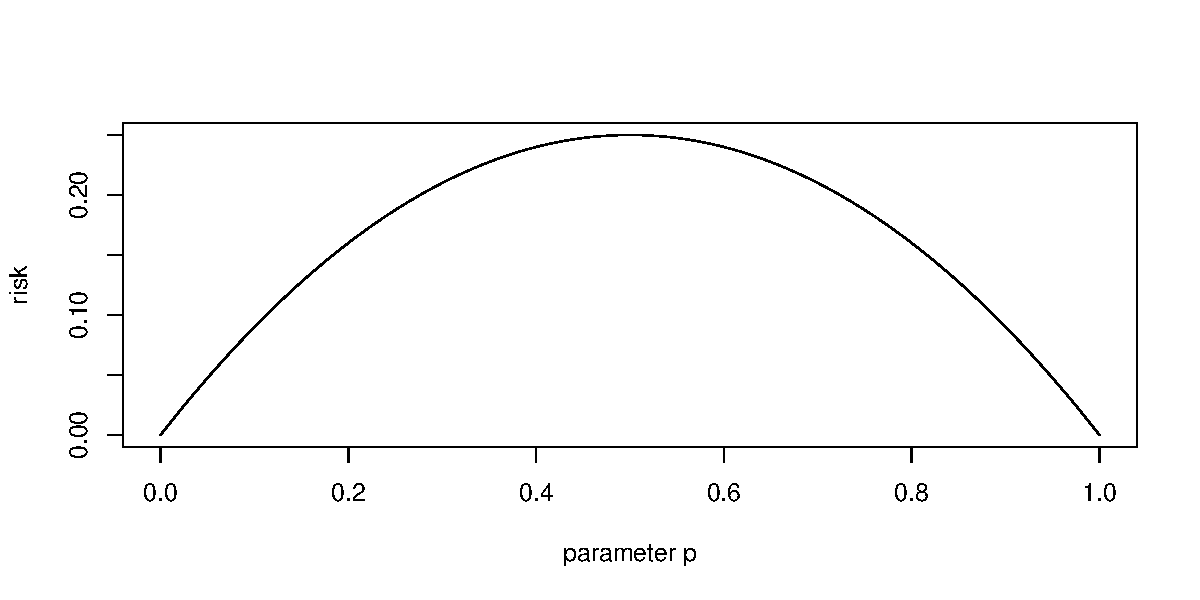
\includegraphics[width=\textwidth]{img/fig02.pdf}
\end{center}

\end{frame}

%%%%%%%%%%%%%%%%%%%%%%%%%%%%%%%%%%%%%%%%%%%%%%%%%%%
\begin{frame}[fragile] \frametitle{}

What about $a = 1/4$ and $b = 3/4$?

\pause Its risk is:
\begin{align*}
\mathbb{E} \mathcal{L} (\theta, \widehat{\theta})
&= \mathbb{P}(X = 0) \cdot (p - a)^2 + \mathbb{P}(X = 1) \cdot (p - b)^2 \\
&= (1-p) \cdot (p - 1/4)^2 + p \cdot (p - 3/4)^2 \\
&= 1 / 16
\end{align*}

\end{frame}

%%%%%%%%%%%%%%%%%%%%%%%%%%%%%%%%%%%%%%%%%%%%%%%%%%%
\begin{frame}[fragile] \frametitle{}

The risk (for squared error loss) of an estimator can
be decomposed into two components, the squared bias and
the variance:
\begin{align*}
\mathbb{E} \mathcal{L} (\theta, \widehat{\theta}) &=
\mathbb{E} (\theta - \widehat{\theta})^2 \\
&= \mathbb{E} (\theta - \mathbb{E}\widehat{\theta} + \mathbb{E}\widehat{\theta} - \widehat{\theta})^2 \\
&=\mathbb{E} (\theta - \mathbb{E}\widehat{\theta})^2 + \mathbb{E} (\widehat{\theta} - \widehat{\theta})^2 \\
&=(\theta - \mathbb{E}\widehat{\theta})^2 + \mathbb{E} (\widehat{\theta} - \mathbb{E}\widehat{\theta})^2 \\
&= \text{Bias}(\widehat{\theta})^2 + \text{Var} (\widehat{\theta})
\end{align*}
\pause In introductory statististics courses, and so far in this course,
we have focused on finding estimators with the minimum variable that have
zero bias. Typically these do not depeend on the actual value of $\theta$.

\end{frame}

%%%%%%%%%%%%%%%%%%%%%%%%%%%%%%%%%%%%%%%%%%%%%%%%%%%
\begin{frame}[fragile] \frametitle{}

\begin{center}
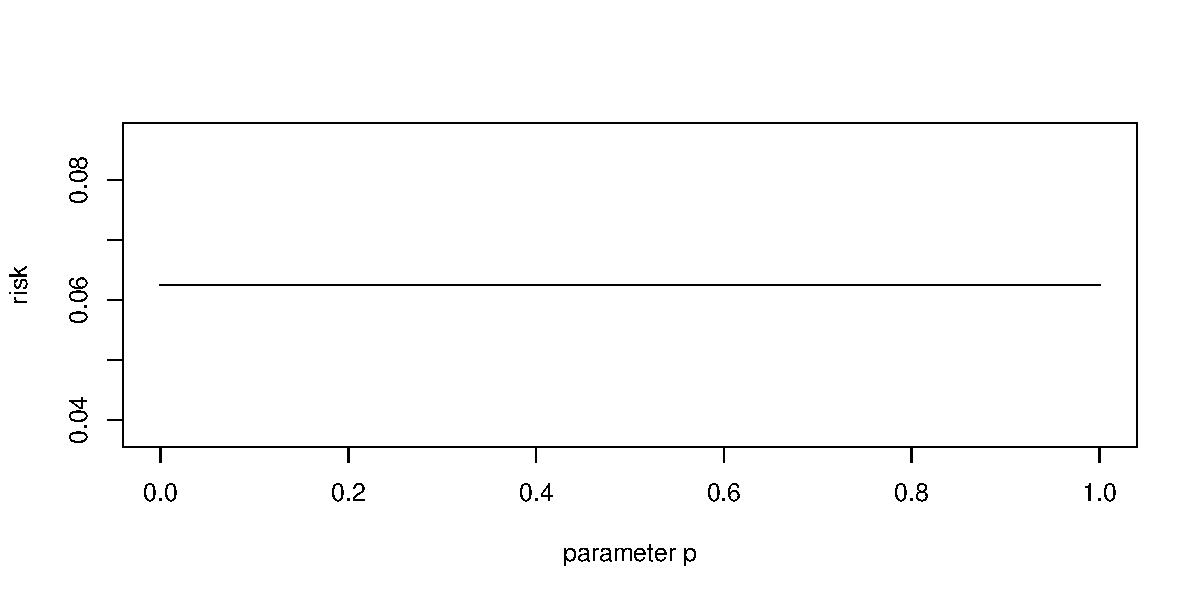
\includegraphics[width=\textwidth]{img/fig03.pdf}
\end{center}

\end{frame}

%%%%%%%%%%%%%%%%%%%%%%%%%%%%%%%%%%%%%%%%%%%%%%%%%%%
\begin{frame}[fragile] \frametitle{}

\begin{flushright}
{\color{yaleblue}\sc\fontsize{1cm}{0cm}\selectfont Back to Linear Models}
\end{flushright}

\end{frame}

%%%%%%%%%%%%%%%%%%%%%%%%%%%%%%%%%%%%%%%%%%%%%%%%%%%
\begin{frame}[fragile] \frametitle{}

On the last problem set I had you define the estimator:
\begin{align*}
\widehat{\beta}_{\alpha} &= \alpha \cdot \widehat{\beta}_{ols}
\end{align*}
And simulated the mean squared error of the resulting estimator.
This was an estimate of the risk of the estimator.

\pause Now, we will try to do this analytically.

\end{frame}

%%%%%%%%%%%%%%%%%%%%%%%%%%%%%%%%%%%%%%%%%%%%%%%%%%%
\begin{frame}[fragile] \frametitle{}

What is the bias of this estimator:
\begin{align*}
\mathbb{E} \left(\beta - \widehat{\beta}_{\alpha} \right) &= \left(\beta - \alpha \cdot \mathbb{E} \widehat{\beta} \right) \\
&= (1 - \alpha) \cdot \beta
\end{align*}

\end{frame}

%%%%%%%%%%%%%%%%%%%%%%%%%%%%%%%%%%%%%%%%%%%%%%%%%%%
\begin{frame}[fragile] \frametitle{}

And the variance is:
\begin{align*}
\mathbb{V} \left( \widehat{\beta}_{\alpha}  \right) &= \alpha^2 \sigma^2 \cdot (X^t X)^{-1}
\end{align*}

\end{frame}

%%%%%%%%%%%%%%%%%%%%%%%%%%%%%%%%%%%%%%%%%%%%%%%%%%%
\begin{frame}[fragile] \frametitle{}

So the risk is equation to:
\begin{align*}
\mathcal{R} (\widehat{\beta}_{\alpha}, \beta) &= (1-\alpha)^2 ||\beta||_2^2 + \alpha^2 \sigma^2 \cdot (X^t X)^{-1}
\end{align*}

\end{frame}

% %%%%%%%%%%%%%%%%%%%%%%%%%%%%%%%%%%%%%%%%%%%%%%%%%%%
% \begin{frame}[fragile] \frametitle{}

% The question is, given a system of linear
% equations:
% \begin{align*}
% A b = y
% \end{align*}
% What does the set of numerically allowable results look
% like?

% \end{frame}

% %%%%%%%%%%%%%%%%%%%%%%%%%%%%%%%%%%%%%%%%%%%%%%%%%%%
% \begin{frame}[fragile] \frametitle{}

% Let $\beta$ be the true solution, calculatable only by a machine
% with perfect precision. Then any other $b$ such that:
% \begin{align*}
% ||Ab - y|| \leq \epsilon
% \end{align*}
% Gives us:
% \begin{align*}
% ||Ab - A\beta|| \leq \epsilon
% \end{align*}

% \end{frame}

% %%%%%%%%%%%%%%%%%%%%%%%%%%%%%%%%%%%%%%%%%%%%%%%%%%%
% \begin{frame}[fragile] \frametitle{}

% So from a prediction standpoint, that is, calculating $Ab$, the
% difference between solutions is not a concern. Howerver, if we
% are interested in
% \begin{align*}
% ||Ab - A\beta|| \leq \epsilon
% \end{align*}

% \end{frame}

\end{document}











